This section aims to give a first analysis of the system.

We will first present the high level entities of the system and then model our use-cases as system level sequence diagrams.

\subsection{High-level entities}
	\label{sec:analysisdiagram}
	Figure~\ref{fig:analysis-model} identifies the high-level entities in the system. We will now explain the functionality of the entities that we chose.

	\begin{description}
		\item[User] \hfill \\
			This class represents all users in the system, regardless of their role in events (organizer/invitee).
		\item[Event] \hfill \\
			Represents an event in the system.
		\item[Response] \hfill \\
			A response from a User about participation in an Event in the system. This is either yes or no and does not specify any date or time.
		\item[DateTimeSlot] \hfill \\
			Represents a date/time.
		\item[Poll] \hfill \\
			A poll that Users can cast Votes on. This is always associated with an event and can not exist on its own. A poll has several DateTimeSlots as options that Users can vote on.
		\item[Vote] \hfill \\
			This class represents a vote on a Poll. A DateTimeSlot is associated with this Vote, representing the date/time that the User voted on.
		\item[dataTracker]
			This class represents a database that tracks all the events and the users in the system.
			
	\end{description}
	
	\begin{figure}[H]
		\centering
		\begin{tikzpicture}
			\begin{class}{User}{0,3}
			\end{class}
		
			\begin{class}{Vote}{4,6}
			\end{class}

			\begin{class}{DateTimeSlot}{4,9}
			\end{class}

			\begin{class}{Poll}{12,3}
			\end{class}

			\begin{class}{Event}{12,0}
			\end{class}

			\begin{class}{Response}{0,0}
			\end{class}

			\begin{class}{dataTracker}{6,3}
			\end{class}

			\association{Response}{}{}{User}{}{}
			\association{Response}{}{}{Event}{}{}
			\association{DateTimeSlot}{}{}{Vote}{}{}
			\association{Vote}{}{}{User}{}{}
			\association{Vote}{}{}{Poll}{}{}
			\association{User}{}{}{Event}{}{}
			\association{User}{}{}{dataTracker}{}{}
			\association{Event}{}{}{dataTracker}{}{}
			\composition{Event}{}{}{Poll}
		\end{tikzpicture}
		\caption{High-level entities in the system}
		\label{fig:analysis-model}
	\end{figure}
	
\subsection{High-level message sequence diagram}
	Figure~\ref{hmsc:all} gives a high-level sequence diagram for our system. It shows how our use-cases relate to each other in a full system overview.

	\begin{figure}[H]
		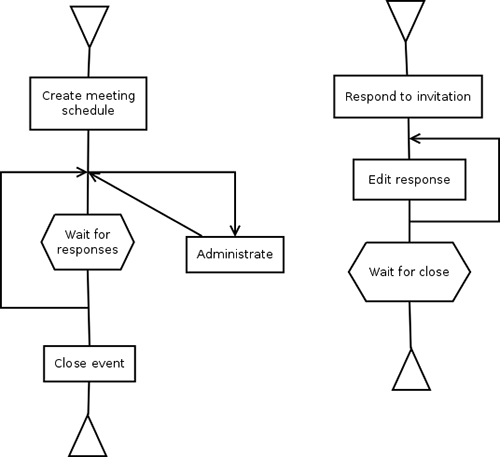
\includegraphics{img/hmsc.png}
		\caption{High-level message sequence diagram}
		\label{hmsc:all}
	\end{figure}

\subsection{System level sequence diagrams}
	%Note: These should be for each use case, with System one entity and entities for the actors
	This section gives system level sequence diagrams for each of the use cases described in section~\ref{sec:usecases} it shows all actors and the system. We chose to model the email service as a separate entity here, because it is not part of our system.
	\begin{figure}[H]
		\centering
		\begin{msc}{Create meeting schedule}
			\declinst{org}{Organizer}{}
			\declinst{inv}{Invitee}{}
			\declinst{sys}{System}{}
			\declinst{email}{Email service}{}

			\mess{Enter event data}{org}{sys}
			\nextlevel

			\mess{Enter date/time option}{org}{sys}
			\nextlevel
	
			\mess{Enter invited people}{org}{sys}
			\nextlevel	

			\mess{Invite people}{org}{sys}
			\nextlevel
			\nextlevel

			\mess{Show event}{sys}{org}
			\nextlevel
			\nextlevel

			\mess{Set poll status and limitations}{org}{sys}
			\nextlevel

			\mess{Submit event}{org}{sys}
			\nextlevel

			\regionstart{coregion}{sys}			
			\nextlevel
			\nextlevel

			\mess{Send confirmation email}{sys}{email}
			\nextlevel
			
			\mess{Send confirmation email}{email}{org}
			\nextlevel
			\nextlevel

			\mess{Send invitation email}{sys}{email}
			\nextlevel
			
			\mess{Send invition email}{email}{inv}
			\nextlevel
			\nextlevel

			\regionend{sys}
			\nextlevel

		\end{msc}
		\caption{Create meeting schedule}
		\label{smsc:createmeeting}
	\end{figure}
	
	We assume that the user is already registered and logged in before the start of this sequence chart. Handling login is out of the scope of this project.

	
	\begin{figure}[H]
		\centering
		\begin{msc}{Respond to meeting invitation}
			\declinst{org}{Organizer}{}
			\declinst{inv}{Invitee}{}
			\declinst{sys}{System}{}
			\declinst{email}{Email service}{}

			\mess{Confirm attendance}{inv}{sys}
			\nextlevel

			\mess{Present options}{sys}{inv}
			\nextlevel
			\nextlevel

			\mess{Vote}{inv}{sys}
			\nextlevel
			\nextlevel

			\mess{Notification}{sys}{email}
			\nextlevel

			\mess{Notification}{email}{org}
			\nextlevel
			\nextlevel

			\mess{Show vote statistics}{sys}{inv}
			\nextlevel
		\end{msc}
		\caption{Respond to meeting invitation}
		\label{smsc:respondmeeting}
	\end{figure}
	
	The same assumption holds for users that receive an invitation. Before this sequence chart starts, users have already completed either a signup process or a login process. Again, specifying these is out of the scope of this project.
	
	This assumption will hold for any of the SMSCs in this section.

	\begin{figure}[H]
		\centering
		\begin{msc}{Edit meeting response}
			\declinst{org}{Organizer}{}
			\declinst{inv}{Invitee}{}
			\declinst{sys}{System}{}
			\declinst{email}{Email service}{}
		
			\mess{Reconfirm attendance}{inv}{sys}
			\nextlevel

			\mess{Present options with previous votes}{sys}{inv}
			\nextlevel
			\nextlevel

			\mess{Vote}{inv}{sys}
			\nextlevel
			\nextlevel

			\mess{Notification}{sys}{email}
			\nextlevel

			\mess{Notification}{email}{org}
			\nextlevel
			\nextlevel

			\mess{Show vote statistics}{sys}{inv}
			\nextlevel

		\end{msc}
		\caption{Edit meeting response}
		\label{smsc:editmeetingresp}
	\end{figure}


	\begin{figure}[H]
		\centering
		\begin{msc}{Administrate event}
			\declinst{org}{Organizer}{}
			\declinst{sys}{System}{}
			
			\mess{Event overview}{sys}{org}
			\nextlevel
			\nextlevel

			\mess{Choose setting to edit}{org}{sys}
			\nextlevel

			\mess*{}{sys}{org}
			\nextlevel
			\nextlevel

			\mess{Edit setting}{org}{sys}
			\nextlevel
		\end{msc}
		\caption{Administrate event}
		\label{smsc:adminevent}
	\end{figure}

	\begin{figure}[H]
		\centering
		\begin{msc}{Close event}
			\declinst{org}{Organizer}{}
			\declinst{sys}{System}{}
			\declinst{email}{Email service}{}
			\declinst{inv}{Invitee}{}
			\declinst{inv2}{Invitee}{}

			\mess{Sure?}{sys}{org}
			\nextlevel
			\mess*{Yes}{org}{sys}
			\nextlevel
			\nextlevel

			\mess{Show date/time options}{sys}{org}
			\nextlevel
			\mess*{Select final date}{org}{sys}
			\nextlevel
			\nextlevel

			\mess{Set optional message}{org}{sys}
			\nextlevel
			\nextlevel

			\mess{Conformation}{sys}{email}
			\nextlevel
		
			\regionstart{coregion}{email}
			\nextlevel
	
			\mess{Confirmation}{email}{org}
			\nextlevel

			\mess{Confirmation}{email}{inv}
			\nextlevel

			\mess{Confirmation}{email}{inv2}
			\nextlevel

			\regionend{email}	

		\end{msc}
		\caption{Close event}
		\label{smsc:closeevent}
	\end{figure}
